\section{Attitude Model} \label{sec:AttitudeModel}
The attitude model of the quadcopter describes how the roll, pitch and yaw angles evolve according to the forces and torques exerted by the propellers. 

The basis for deriving the model are the free body diagrams illustrated in \autoref{fig:droneDiagram} and \ref{fig:torquesDiagram}. 

\begin{minipage}{\linewidth}
	\begin{minipage}{0.6\linewidth}
		\begin{figure}[H]
			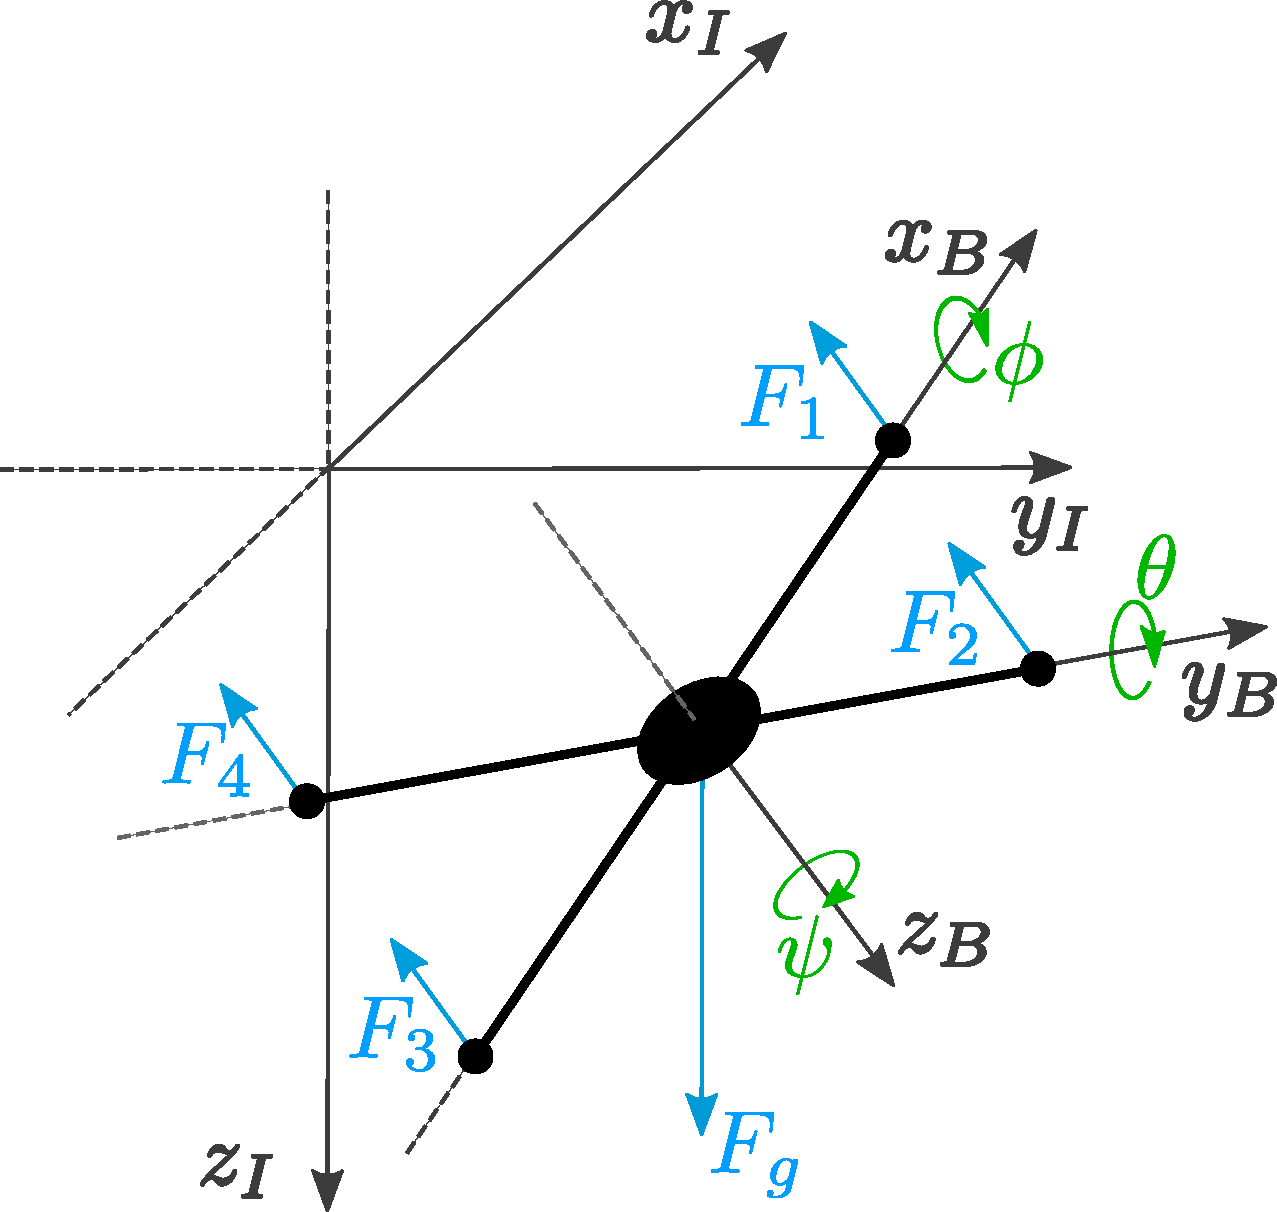
\includegraphics[scale=.4]{figures/droneDiagram}
			\centering
			
			\captionof{figure}{Free body diagram that holds both the inertial and body reference systems, as well as the references for the angles, roll, pitch and yaw.}
			\label{fig:droneDiagram}
		\end{figure}
	\end{minipage}
	\hspace{0.03\linewidth}
	\begin{minipage}{0.35\linewidth}
		\begin{figure}[H] \vspace{20mm}
			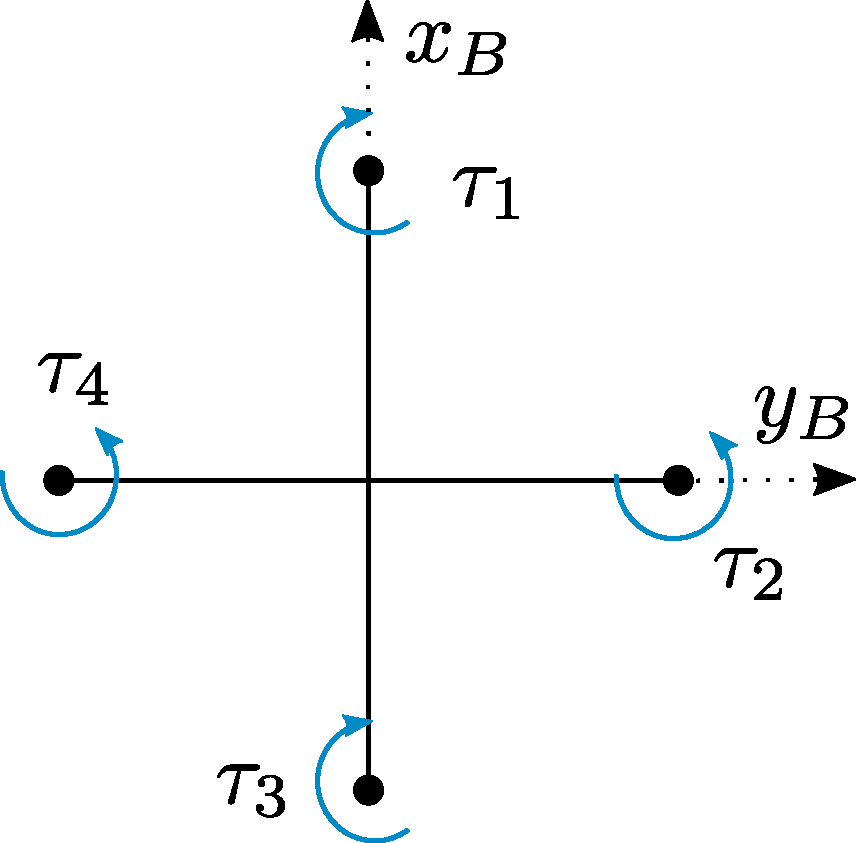
\includegraphics[scale=.4]{figures/torquesDiagram}
			\centering
            \vspace{10mm}
			\captionof{figure}{Free body diagram with the references for the torques produced by the drag forces at the propellers.}
			\label{fig:torquesDiagram}
		\end{figure}
	\end{minipage}
\end{minipage}

From the diagrams above, the equations of angular motion along the three body axes can be derived by first principles modeling, that is, using only laws of physics. In this case, Newton's Second Law for rotational motion, as seen in \autoref{eq:newtonangular}.
%
\begin{align}
	J\cdot\alpha=\sum\tau
	\label{eq:newtonangular}
\end{align}
\begin{where}
\va{J}{is the moment of inertia}{kg \cdot m^2}
\va{\alpha}{is the angular acceleration}{rad\cdot s^{-2}}
\va{\tau}{are the torques applied to the system}{N \cdot m}
\end{where}

%\begin{where}
%	\va{J}{is the moment of inertia}{kg\cdot m^2}
%	\va{\alpha}{is the angular acceleration}{rad\cdot m\cdot s^{-2}}
%	\va{\tau_i}{are the torques applied to the system}{Nm}
%\end{where}
%It shall be noted, that the fact that Newton's laws, that only apply in relation to an inertial reference, are applied even though the earth is accelerating and rotating, as it is the assumption, that it is of little influence for the system of the quadcopter. 
%
From applying Newton's Second Law, \autoref{eq:AngleEq1}, \ref{eq:AngleEq2} and \ref{eq:AngleEq3} are obtained. As it can be seen, the roll and pitch angular accelerations depend on the thrust forces exerted by the propellers placed along the y- and x-axis of the quadcopter, respectively. The yaw angle changes due to the torques created by the drag forces in the propellers.
%
\begin{align}
	J_x\cdot\ddot{\phi}&=(F_4-F_2)\cdot L  \label{eq:AngleEq1} \\
	J_y\cdot\ddot{\theta}&=(F_1-F_3)\cdot L  \label{eq:AngleEq2}\\
	J_z\cdot\ddot{\psi}&=\tau_1-\tau_2+\tau_3-\tau_4
	\label{eq:AngleEq3}
\end{align}
\begin{where}
\va{J_x}{is the inertia around the x axis}{kg\cdot m^2}
\va{J_y}{is the inertia around the y axis}{kg\cdot m^2}
\va{J_z}{is the inertia around the z axis}{kg\cdot m^2}
\va{\ddot{\phi}}{is the roll angular acceleration}{rad\cdot s^{-2}}
\va{\ddot{\theta}}{is the pitch angular acceleration}{rad\cdot s^{-2}}
\va{\ddot{\psi}}{is the yaw angular acceleration}{rad\cdot s^{-2}}
\va{F_i}{is the thrust force from each propeller}{N}
\va{L}{is the length from center of mass to motor}{m}
\va{\tau_i}{is the drag torque from each propeller}{N \cdot m}
\end{where}

%\begin{where}
%\va{\ddot{\phi}}{is roll angular acceleration}{rad $\cdot$ s$^{-2}$}
%\va{\ddot{\theta}}{is  pitch angular acceleration}{rad$\cdot$ s$^{-2}$}
%\va{\ddot{\psi}}{is yaw angular acceleration}{rad$\cdot$ s$^{-2}$}
%\va{J_x}{is the body moment of inertia around $x_B$ direction}{kg $\cdot$ m$^2$}
%\va{J_y}{is the body moment of inertia around $y_B$ direction}{kg $\cdot$ m$^2$}
%\va{J_z}{is the body moment of inertia around $z_B$ direction}{kg $\cdot$ m$^2$}
%\va{L}{is the length of the arm of the quadcopter}{m}
%\va{F_n}{is the thrust force produced in each propeller}{N}
%\va{\tau_n}{is the torque due to the drag force in each propeller}{Nm}
%\end{where}
The thrust forces and drag torques from the propeller can be assumed to be proportional to the square of the velocity of the motor, related by constants obtained as described in \autoref{app:ThrustTest} and \ref{app:TorqueTest}. The equations above can be rewritten to include these terms.
%
\begin{align}
J_x\cdot\ddot{\phi}&=k_{th} \cdot(\omega^2_4-\omega^2_2) \cdot L \label{eq:AngleEqVelocities1}\\
J_y \cdot\ddot{\theta}&=k_{th} \cdot(\omega^2_1-\omega^2_3) \cdot L \label{eq:AngleEqVelocities2} \\
J_z\cdot\ddot{\psi}&=k_d \cdot(\omega^2_1-\omega^2_2+\omega^2_3-\omega^2_4)
\label{eq:AngleEqVelocities3}
\end{align}
\begin{where}
\va{k_{th}}{is the thrust constant}{N\cdot s^2 \cdot rad^{-2}}
\va{k_d}{is the drag constant}{N \cdot m\cdot s^2 \cdot rad^{-2}}
\end{where}

\autoref{eq:AngleEqVelocities1}, \ref{eq:AccelerationEqInertialVelocities2} 
and \ref{eq:AccelerationEqInertialVelocities3} are the final attitude model expressions that are brought forward. %Now that the attitude model is known, the translational model must be derived. This is done in the following section. 